\documentclass[11pt]{amsart}
\usepackage{geometry}                % See geometry.pdf to learn the layout options. There are lots.
\geometry{letterpaper}                   % ... or a4paper or a5paper or ... 
%\geometry{landscape}                % Activate for for rotated page geometry
%\usepackage[parfill]{parskip}    % Activate to begin paragraphs with an empty line rather than an indent
\usepackage{graphicx}
\usepackage{amssymb}
\usepackage{amsmath}
\usepackage{epstopdf}
\usepackage{algorithm}
\usepackage{hyperref}
\usepackage[noend]{algpseudocode}
\DeclareGraphicsRule{.tif}{png}{.png}{`convert #1 `dirname #1`/`basename #1 .tif`.png}
\makeatletter
\def\BState{\State\hskip-\ALG@thistlm}
\makeatother

\title{Particle Filter Lab}
\author{Matt Barnes}
\date{October 7, 2014}                                           % Activate to display a given date or no date

\begin{document}
\maketitle
\section{Problem Statement}
The goal of this lab is to localize an indoor mobile robot in Wean Hall given a map, laser scans, and odometry readings. A particle filter -- also known as sequential importance resampling -- is the general approach. Though the framework is straightforward, specifics of the motion and sensor models play an essential role in successful localization. I consider trade-offs between robustness, computational efficiency, and accuracy when designing the various components. Two experiments successfully demonstrate localization in Wean Hall.

\section{Approach}
Particle filters are variants of Bayes Filters with an additional resampling process. They can be summarized as an iterative process involving three major steps:

\begin{enumerate}
\item Updating particle positions by sampling from the motion model $p(x_t | u_t, x_{t-1})$
\item Calculating observation probability $w_t$ for each particle using the sensor model $p(z_t | x_t)$
\item Resampling particles with probability $\alpha$ $w_t$
\end{enumerate}

For the case of 2D robot localization, steps 1 and 3 are relatively trivial. Even with a conditional independence assumption enabling the use of occupancy maps, calculating the sensor model probability is the most challenging aspect of the particle filter.

\subsection{Motion Model}
The motion model I used is adapted from \cite{thrun2005probabilistic}. Given odometry readings in standard local coordinates, the model breaks movement into three steps with separate noise. The first step, $\delta_{rot1}$ orients the robot from its heading at time $t-1$ to point at the new position at time $t$. The second step $\delta_{trans}$ moves the robot along its new heading to the position at time $t$. The final step $\delta_{rot2}$ orients the robot to the correct final heading. Together, these three steps move the robot from its initial to final state. The algorithm and noise at each step are shown in Algorithm \ref{motion_model}.

\begin{algorithm}
\caption{sample\_motion\_model\_odometry($u_t, x_{t-1}$)}\label{motion_model}
\begin{algorithmic}
\State $\delta_{rot1} \gets \text{atan2}(\bar y' - \bar y, \bar x' - \bar x) - \bar \theta$
\State $\delta_{trans} \gets \sqrt{(\bar x - \bar x')^2 + (\bar y - \bar  y')^2}$
\State $\delta_{rot2} \gets \bar \theta' - \bar \theta - \delta_{rot1}$
\vspace{1em}

\State $\hat \delta_{rot1} \gets \delta_{rot1} - \text{\bf{sample}}(\alpha_1\delta_{rot1}^2 + \alpha_2\delta_{trans}^2)$
\State $\hat \delta_{trans} \gets \delta_{trans} - \text{\bf{sample}}(\alpha_3\delta_{trans}^2 + \alpha_4\delta_{rot1}^2 + \alpha_4\delta_{rot2}^2)$
\State $\hat \delta_{rot2} \gets \delta_{rot2} - \text{\bf{sample}}(\alpha_1\delta_{rot2}^2 + \alpha_2\delta_{trans}^2)$
\vspace{1em}

\State $x' \gets x + \hat \delta_{trans}\cos(\theta + \hat \delta_{rot1})$
\State $y' \gets y + \hat \delta_{trans}\sin(\theta + \hat \delta_{rot1})$
\State $\theta' \gets \theta + \hat \delta_{rot1} + \hat \delta_{rot2}$
\vspace{1em}

\text{return} $x', y', \theta'$
\end{algorithmic}
\end{algorithm}

Without ground truth, I tuned the parameters $\alpha_1, \alpha_2, \alpha_3, \text{and } \alpha_4$ by hand. I conducted a rough stand-alone tuning using synthetic data along a straight line. $\alpha_1 \text{ and } \alpha_2$ influence rotation and $\alpha_3 \text{ and } \alpha_4$ influence translation. Once the sensor model was finished, I initialized particles in the correct starting region and did a final tuning by examining when failure occurred. All final experiments used values of $\alpha_1 = 0.001, \alpha_2 = 0.001, \alpha_3 = 0.1, \alpha_4 = 0.1$.

\subsection{Sensor Model}
Designing the sensor model was much more interesting because of the number of potential approaches. I tried two very different techniques. The first approach used the ray casting algorithm in \cite{thrun2005probabilistic}. For each laser range reading (of every particle, at each time step), the expected reading is estimated by `casting' out a ray on the known map and returning the distance to the first encountered obstacle. I used a discrete sampling along the ray, somewhere on the order of 5cm -- half the resolution of the map. Missing obstacles is possible by `skipping' over cell corners, but negligible since obstacles are usually large. The returned ray distance $z_t^*$ and actual measurement $z_t$ are fed into sensor model $p(z_t | z_t^*)$. Using the conditional independence assumption of laser scans, the particle's sensor reading probability is the product of the beams' probabilities.

The model $p(z_t | z_t^*)$ considers not only expected sensor noise, but also unexpected objects, max value readings, and random measurements. I used a weighted average of four functions, $p_{hit}(z_t | z_t^*)$, $p_{short}(z_t | z_t^*)$, $p_{max}(z_t | z_t^*)$ and $p_{rand}(z_t | z_t^*)$.

\begin{displaymath}
   p_{hit}(z_t | z_t^*) = \left\{
     \begin{array}{lr}
       \eta \frac{1}{\sqrt{2\pi \sigma_{hit}^2}}e^{-\frac{1}{2}\frac{(z_t - z_t^*)^2}{\sigma_{hit}^2}} & \text{if } 0 \leq z_t \leq z_{max}\\
       0 & \text{otherwise}
     \end{array}
   \right.
\end{displaymath}
\begin{displaymath}
   p_{short}(z_t | z_t^*) = \left\{
     \begin{array}{lr}
       \eta \lambda_{short}e^{-\lambda_{short}z_t} & \text{if } 0 \leq z_t \leq z_t^*\\
       0 & \text{otherwise}
     \end{array}
   \right.
\end{displaymath}
\begin{displaymath}
   p_{max}(z_t | z_t^*) = \left\{
     \begin{array}{lr}
       1 & \text{if } z_t = z_{max}\\
       0 & \text{otherwise}
     \end{array}
   \right.
\end{displaymath}
\begin{displaymath}
   p_{rand}(z_t | z_t^*) = \left\{
     \begin{array}{lr}
       \frac{1}{z_{max}} & \text{if } 0 \leq z_t \leq z_{max}\\
       0 & \text{otherwise}
     \end{array}
   \right.
\end{displaymath}
where $\eta$ is a normalizer to make the probability functions sum to 1. 

I implemented this algorithm in Python and the resulting sensor model with hand tuned weights is shown in Figure 1. I quickly realized ray casting is slow for a large number of particles, even with other tricks such as downsampling laser range readings. Instead of implementing it in C++ or precomputing a look-up table, I tried another much faster approach.
\begin{figure}[t]
\centering
	\label{sensor_model}
        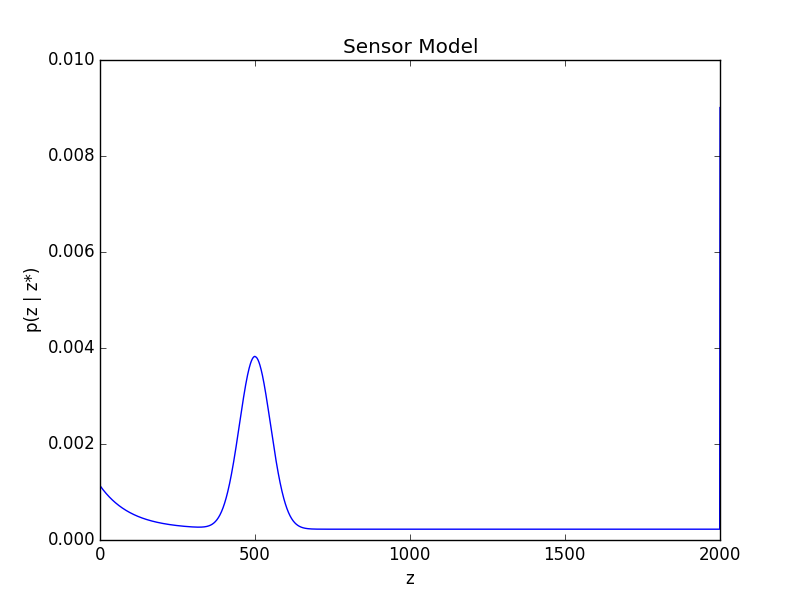
\includegraphics[totalheight=8cm]{sensor_model.png}
        \caption{Sensor model $p(z_t | z_t^*)$, with $z_{max}$ truncated to 2000 for visualization purposes}
\end{figure}

My second approach modeled some of the sensor noise, but did not use ray tracing. I applied a Gaussian filter with $\sigma = 5$ to the map image and looked up the occupancy probability for each laser reading, as shown in Figure \ref{gaussian_map}. This is \emph{much} faster than using ray tracing and requires \emph{no} pre-computations, aside from the trivial Gaussian filter. The Gaussian filter acts as the expected measurement noise, somewhat similar to $p_{hit}$. By setting a minimum threshold on occupancy probability of $p(z_t | z_t^*) \geq 0.01$ and checking for maximum sensor readings, this approach also captured $p_{rand}$ and $p_{max}$. The major drawback of this approach is close unexpected objects are not considered, such as the person who ALWAYS walked in front of the robot.

\begin{figure}[t]
\centering
	\label{gaussian_map}
        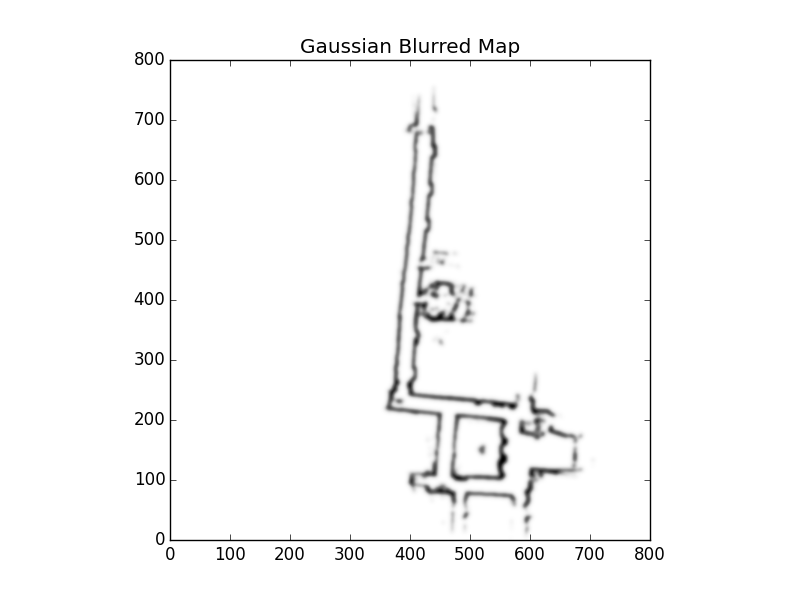
\includegraphics[totalheight=8cm]{gaussian_map.png}
        \caption{Map with Gaussian blur used for fast laser scan look-up}
\end{figure}


\emph{The Not-So-Pretty:}
This algorithm worked as is. However, I introduced several minor `hacks' to improve performance. First, I only initialized particles in completely unoccupied areas (i.e. the halls), a reasonable assumption. This reduced the number of required particles severalfold. I also introduced some uncertainty in the sensor model by raising each beam probability to the power $\alpha = 0.75$. Finally, I subsampled the beams to every 5 degrees.

\section{Results}
\begin{itemize}
\item Video results are publicly available at:
 
\url{https://www.youtube.com/watch?v=4OdnX31wfkU}.
\item The open source code is available at:

 \url{https://github.com/mbarnes1/particle_filter}.
\end{itemize}
The first video (\verb!datalog5.dat!) shows a run that worked almost flawlessly. The filter converges in only a couple time steps and continues to track the robot over the entire experiment. The second video (\verb!datalog1.dat!), demonstrates a case where the filter had trouble converging, but ultimately was able to localize. The non-ray-casting algorithm is biased towards highly occupied areas, as it only samples where the laser reading occurred -- not along the path to it. However, the algorithm clearly still works very well.

Standard experiments using 1000 particles read all the data files, ran the particle filter, and wrote a video file in ~150 seconds. The production quality experiments used 10000 particles and ran proportionally slower.

\subsection{Future Work}
If I were to do this lab again, I'm very intrigued by the idea of precomputing ray casts at all hallway positions and angles. Though I imagine this would take several hours, the actual hash-table lookup would be very fast. My algorithm, implemented in Python, was already able to run close to real-time. With a C++ implementation and the precomputed tables, I imagine the particle filter could be \emph{very} fast and have better convergence.

\bibliography{mybib}{}
\bibliographystyle{ieeetr} 

\end{document}  